\begin{surferPage}[Octica-Chmutov]{Octica lui Chmutov}
    O caracterstic\u{a} atr\u{a}g\u{a}toare la octica lui Chmutov $\text{Chm}_{d}, \ d=8,$
    este simetria ei. Acest lucru poate fi v\u{a}zut \c{s}i prin inspectarea ecua\c{t}iei:
    \[\text{Chm}_{d}\colon T_d(x) + T_d(y) + T_d(z) + 1 = 0,\]
    unde $T_d$ este a\c{s}a-numitul polinom Tchebychev (imaginea din st\^{a}nga).
    Curba $T_8 (x) + T_8 (y) = 0$ este reprezentat\u{a} \^{i}n dreapta:
    
     \begin{center}
      \begin{tabular}{c@{\quad}c}
        \begin{tabular}{c}
          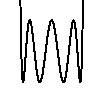
\includegraphics[height=1.75cm]{./../../common/images/Tcheb_008.pdf}
        \end{tabular}    
        &
        \begin{tabular}{c}
          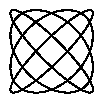
\includegraphics[height=1.75cm]{./../../common/images/Tcheb_2d_008.pdf}
        \end{tabular}    
      \end{tabular}
    \end{center}
    \vspace{-0.3cm}
    Etapele necesare pentru a trece de la aceste imagini la forma suprafe\c{t}ei din
    cititorul interactiv nu este foarte dificil.
    
 Aceste ecua\c{t}ii au fost date de S.V.\ Chmutov la \^{i}nceputul anilor '80.
    La acea vreme, au constituit recordul mondial pentru $\mu(d)$ pentru aproape toate gradele $d$.
    \^{I}n anii '90, Chmutov \c{s}i-a \^{i}mbun\u{a}t\u{a}\c{t}it propriul record, iar \^{i}n 2005, S. ~ Breske,
    O. ~ Labs \c{s}i D. ~ van ~ Straten au adaptat aceast\u{a} construc\c{t}ie pentru a ob\c{t}ine
    suprafe\c{t}e reale av\^{a}nd doar singularit\u{a}\c{t}i reale.
    
\end{surferPage}